\documentclass[12pt,a4paper]{article}

% Packages
\usepackage[T1]{fontenc}
\usepackage[utf8]{inputenc} % optional for modern LaTeX, kept for compatibility
\usepackage{amsmath,amsfonts,amssymb}
\usepackage{amsthm}
\usepackage{graphicx}
\usepackage{geometry}
\usepackage{cite}
\usepackage{placeins}
\usepackage{verbatim}
\usepackage{enumitem}
\usepackage{bbm}
\usepackage{xcolor}
\usepackage{tikz}
\usepackage{hyperref}
\graphicspath{{IMAGES/}}

% Page layout
\geometry{margin=1in}

% Theorem environments
\newtheorem{theorem}{Theorem}[section]
\newtheorem{lemma}[theorem]{Lemma}
\newtheorem{proposition}[theorem]{Proposition}
\newtheorem{corollary}[theorem]{Corollary}
\newtheorem{example}{Example}[section]

\begin{document}

% ---------------- Title Page ----------------
\begin{titlepage}
\centering
\vspace*{1cm}

{\LARGE\bfseries Report on Pattern Identification of Critical Combustion Events}\\[1cm]
{\large VERSION 1.0}\\[0.5cm]
{\large \today}\\[1cm]

\vfill

\begin{flushleft}
{\large\textbf{Abstract}}\\[0.5cm]
This report presents methodologies for pattern identification in critical combustion events.
The work focuses on the development and application of advanced data analysis techniques
to understand and predict combustion instabilities and critical phenomena in reactive
flow systems.
\end{flushleft}

\vfill

\begin{center}
\textbf{Authors:}\\
Isacco Faglioni*\\
Soledad le Clainche\\
Laura Saavedra\\[0.5cm]

\textbf{Reviewer:}\\
Alessandro Parente
\end{center}

\vfill

\begin{center}
{\small DELIVERABLE PROJECT}\\
{\small \today}
\end{center}

\end{titlepage}

% ---------------- Main Content ----------------
\tableofcontents
\newpage

\section{Introduction}
\begin{comment}
Understanding critical combustion events is a complex task that involves extensive analysis of both experimental and numerical data. Finding patterns in these datasets is an important step towards building better models for combustin phoenomena. 
 Many tools exist both in the reactive and non reactive flows. Proper Orthogonal Decomposition (POD) (CITAZIONE), is an Singular Value Decomposition (SVD) based method that provide a low rank rappresentation of the flow rewriting it as a sum of orthogonal spatial patterns.
 Principal component analysis has been successfully employed to project high-dimensional data onto a lower-dimensional orthogonal subspace of thermodynamical variables (CITAZIONE), effectively reducing the complexity of the system while retaining its essential features. However, this method is not able to capture the temporal evolution of the system and it is not able to provide a physical interpretation of the modes.
 Dynamic Mode Decomposition (DMD) (CITAZIONE) allows the reduction of the system in spatio-temporal modes which have both a spatial structure and an associated temporal frequency and growth rate. Thus the system is rapresented as the sum of modes evolving with a linear dynamics in time that allows the study of the spectral properties of the sytesm. Although powerful this method suffers from noisy data and it oftern is inadequate to provide an accurate description of turbulent reactive flows. High Order Dynamic Mode Decomposition (HODMD) (CITAZIONE) is a extention of DMD that improves the method by introducing the higher order Koopman hypothesis. This makes it more robust and has already been succesfully applied in reactive flows (CITAZIONE)
Combustion data often presents itself in tensorial form. Moreover the most valuable datases, i.e. the ones that most closely represent the real physics of the system, are often the ones with the highest dimensionality both in spatial component and in the number of variables. This has sparked interest in methods that process data directly into this form and don't require reshaping into matrix form as in the case of SVD based methods and DMD.

The current report focuses on describing the application of these techniques to enhance the algorithms that allows patter identification in combustion data. High Order Singular Value Decomposition (CITAZIONE), a generalization of SVD, is discussed as a tool to both compress and extract physical patterns from huge combustion datasets. In particular, this method allows for multi modal analysis along each axis of the tensor at the same time, allowing to quantify the importance of each dimension of the tensor.  
When combined with HODMD this, allows for identification of key feature in the dynamics of the reactive flow.

Furthermore, 

%eseguendo una riduzione della dimensionalità indipendente lungo ciascun modo del tensore — dimensioni spaziali, temporali e delle variabili — consentendo migliori tassi di compressione e un filtraggio del rumore più mirato. Combinata con l'HODMD, l'HOSVD fornisce un framework multi-dimensionale naturale per analizzare le dinamiche complesse e multi-scala dei flussi reattivi. Per arricchire ulteriormente l'interpretazione fisica di queste decomposizioni, la Decomposizione di Koopman Spazio-Temporale (STKD) [Le Clainche et al., 2020] estende l'HODMD al dominio spaziale, identificando pattern di onde viaggianti caratterizzati sia da frequenze che da numeri d'onda. Ciò consente di rappresentare il flusso come sovrapposizione di strutture propaganti, offrendo una comprensione più profonda dell'interazione tra dinamiche spaziali e temporali nella combustione turbolenta. Al di là degli approcci basati sulla decomposizione, modelli surrogati data-driven come la Regressione con Processi Gaussiani (GPR) [Rasmussen & Williams, 2006] offrono una prospettiva complementare, consentendo la ricostruzione probabilistica e la predizione dei campi di flusso a partire da osservazioni sparse. Quando estesa con la riduzione della dimensionalità basata su HOSVD, la GPR può operare in uno spazio tensoriale compresso, rendendola scalabile agli dataset ad alta dimensionalità generati da DNS e LES, preservando al contempo le capacità di quantificazione dell'incertezza. In questo lavoro, applichiamo ed estendiamo queste metodologie — HOSVD, HODMD, GPR potenziata con HOSVD e STKD — a dataset di combustione DNS e LES, con l'obiettivo di fornire un framework efficiente, fisicamente interpretabile e computazionalmente trattabile per l'analisi della dinamica dei flussi reattivi.

\end{comment}
\section{Datasets}
\label{sec:datasets}

Data for this report comes from different members of the consortium. The first dataset, is the one anticipated in the previous deliverable on data assimilation. It is generated by Giovanni Grassi (DC6) at CORIA and descibes a Hydrogen-Ammonia blend. This data contains different boundry conditions, making it suitable for pattern identification within the same phoenomena across different scenatios. Moreover the study of the behaviour of combustion of Hydrogen-Ammonia blends is extremely important in the scope of reducing NOx emission, one of the main objectives of the overall project.     
The second dataset is generated by Lorenzo Fracino (DC2) at RWTH Aachen and rapresents a Mehtane-Hydrogen mixing layer.  
\subsection{NH$_3$/H$_2$ non-premixed mixing layer}
\label{sec:DATA_CORIA}

This dataset consists of direct numerical simulations (DNS) of a two-dimensional non-premixed ammonia-hydrogen-air reacting mixing layer. It is generated by DCGIOVANNI at CORIA using the structured mesh reactive flow solver SiTCom-B \cite{sitcomb}. The configuration represents a splitter-plate stabilized flame in which a cold fuel stream and a hot air stream interact across a shear layer, representative of conditions encountered in practical burners. 


The lower stream consists of a NH$_3$/H$_2$ fuel blend (with 15\% H$_2$ by volume) at ambient temperature (300~K) with a mean velocity of 15~m~s$^{-1}$, while the upper stream consists of preheated air with a mean velocity of 39.6~m~s$^{-1}$. A cold wall maintained at 600~K is imposed at the top boundary, and a symmetry condition is applied at the bottom. Homogeneous velocity fluctuations of 10\% are prescribed at both inlets. The computational domain measures $12 \times 1$~cm and is discretized on a uniform grid of $2400 \times 200$ cells with a resolution of 50~$\mu$m. 

\FloatBarrier
\begin{figure}[htbp]
    \centering
    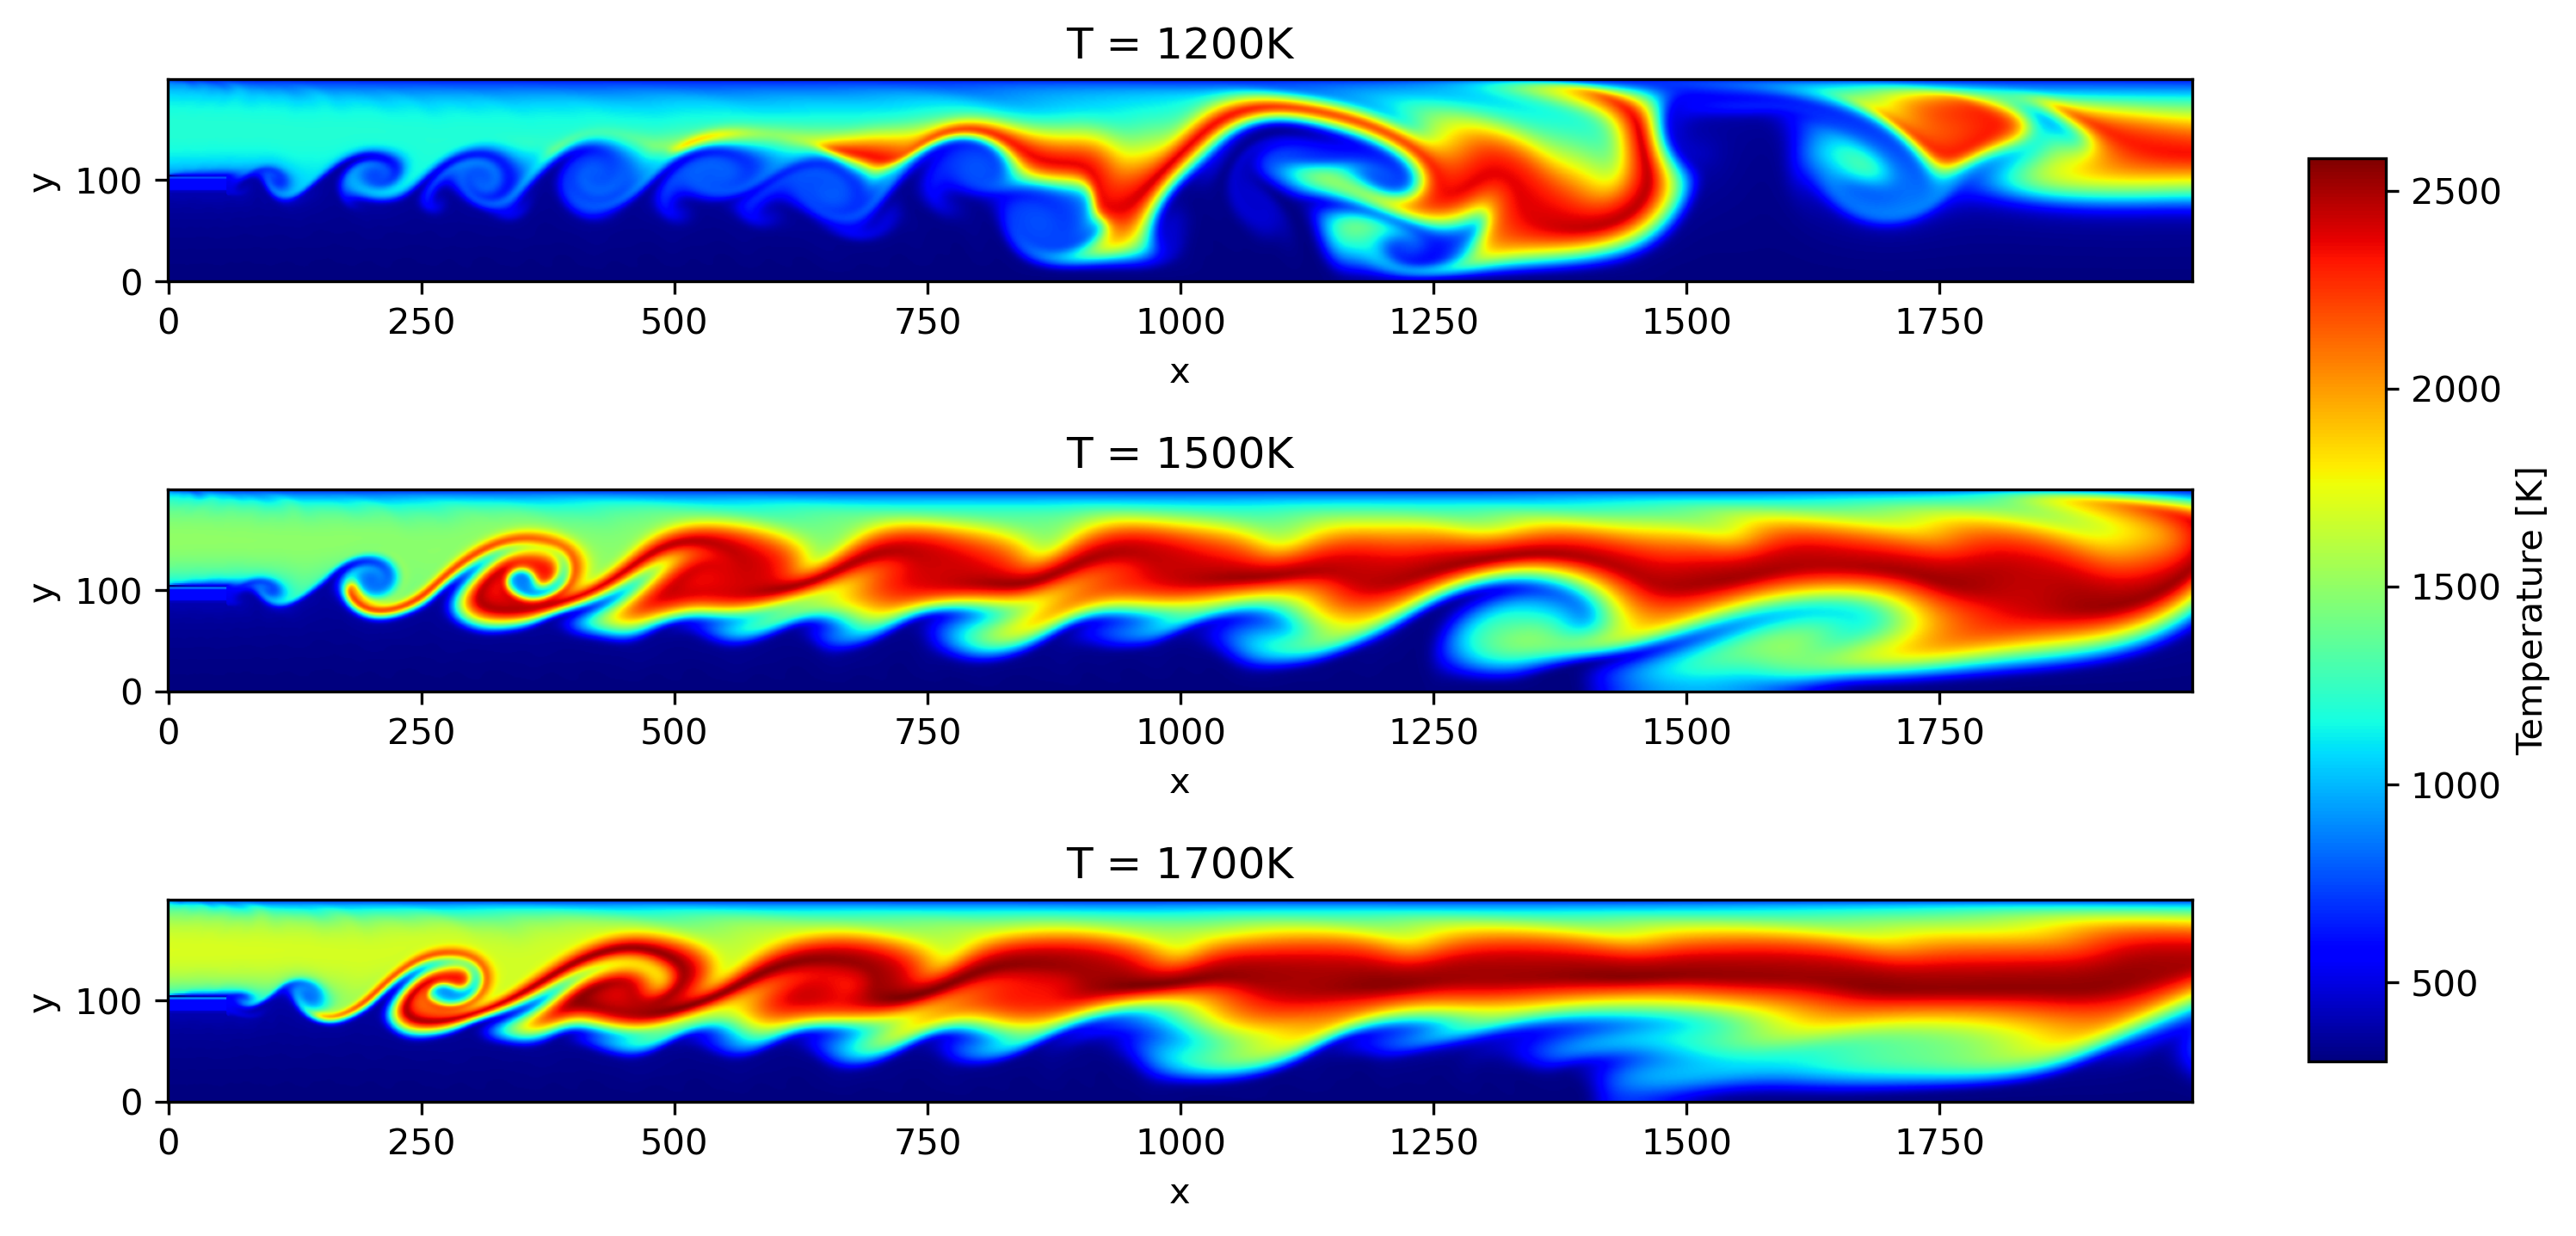
\includegraphics[width=0.85\textwidth]{../IMAGES/DATASETS/coria_3snap.png}
    \caption{Three representative snapshots of the temperature field from the NH$_3$/H$_2$ non-premixed reacting mixing layer DNS, illustrating the spatial evolution of the flame and mixing structures at different instants.}
    \label{fig:coria_data}
\end{figure}
\FloatBarrier

Three datasets are generated at different air preheat temperatures, namely 1200~K, 1500~K, and 1700~K, to probe the sensitivity of the flame dynamics and species evolution to the inlet thermal boundary condition. The domain geometry, grid resolution, and flow velocities are identical across all three cases. Each snapshot contains 19 reactive scalar fields corresponding to the species of the reduced mechanisms RmAH-1 and RmAH-2 \cite{grassi2025} — namely H$_2$, O$_2$, H$_2$O, H, O, OH, HO$_2$, NH$_3$, NH$_2$, NH, N, NO, NO$_2$, N$_2$O, HNO, NNH, N$_2$H$_2$, N$_2$, and Ar — together with temperature, yielding 20 variables in total. The species analysis presented in this work is conducted exclusively on the 1500~K dataset, which constitutes the reference operating condition for the assessment of the proposed methodologies.
\begin{comment}
    
\subsection{CH$_4$/H$_2$ MILD combustion mixing layer}
\label{sec:DATA_RWTH}

This dataset consists of direct numerical simulations (DNS) of a temporally evolving three-stream mixing layer representative of MILD (Moderate or Intense Low-oxygen Dilution) combustion conditions. It is generated at the Institute for Combustion Technology of RWTH Aachen University using the in-house finite-difference solver CIAO \cite{frascino2025}, which solves the reactive unsteady Navier--Stokes equations in the low-Mach-number limit. The full dataset and its physical analysis are described in detail in \cite{frascino2025}.


The configuration consists of three co-flowing streams: a central cold fuel jet of 25\%~H$_2$/75\%~CH$_4$ (by volume) at $T_\mathrm{fuel} = 300$~K, flanked by two jets of preheated air at $T_\mathrm{air} = 900$~K, which are in turn surrounded by streams of lean hot combustion products at $T_\mathrm{hot} = 1225$~K. The equivalence ratio of the mixture is $\phi = 0.8$. Periodic boundary conditions are imposed in the streamwise ($x$) and spanwise ($z$) directions, while an outlet condition is applied in the cross-stream ($y$) direction. The DNS is initialised from 1D flamelet profiles mapped onto a smooth mixture-fraction field, placing the simulation in a quasi-frozen state that allows the onset of autoignition to be captured. The chemical kinetics are described by a reduced mechanism for lean CH$_4$/H$_2$ combustion comprising 24 species and 251 reactions, derived from the full C3MechV3.3 model \cite{dong2022}.

The dataset comprises four cases obtained by independently varying two Damk\"{o}hler numbers: $Da_\mathrm{HA}$, associated with the hot-products--air mixing process, and $Da_\mathrm{FA}$, associated with fuel--air mixing. High $Da_\mathrm{HA}$ values correspond to high-dilution (HD) conditions characteristic of the MILD regime, while low $Da_\mathrm{HA}$ values correspond to low-dilution (LD), non-MILD conditions. Each dilution condition is combined with a fast ($Da_\mathrm{FA}$ low) or slow ($Da_\mathrm{FA}$ high) fuel--air mixing rate, yielding the four cases HD-FF, HD-SF, LD-FF, and LD-SF. The computational grid contains approximately $1.2 \times 10^9$ cells for the HD cases and $0.7 \times 10^9$ cells for the LD cases, with a minimum of 10 grid points resolved across the OH reaction layers and a ratio $\Delta/\eta < 2$ ensuring that the Kolmogorov scale is well resolved throughout the domain.

\subsubsection*{Filtered DNS}

The data used in the present work is not the raw DNS output but a spatially filtered version of it, obtained by applying a box filter of width $\Delta_f = 8\,\Delta_\mathrm{DNS}$ to the DNS fields, where $\Delta_\mathrm{DNS}$ denotes the local DNS grid spacing. This filtered DNS (fDNS) retains the large-scale coherent structures and the dominant dynamical features of the flow while suppressing the smallest dissipative scales, making the dataset tractable for the tensor-based analysis described in Section~\ref{sec:methods}.

% -------------------------------------------------------
% TODO — ask the data provider (Lorenzo Frascino / RWTH):
%   1. Which of the four cases (HD-FF, HD-SF, LD-FF, LD-SF) are available?
%   2. Confirm filter type: box filter (top-hat) with Delta_f = 8 * Delta_DNS?
%   3. What variables are provided? (temperature + all 24 species, or a subset?)
%   4. Number of snapshots and temporal spacing Delta_t for each case?
% -------------------------------------------------------
\end{comment}

\subsection{ULB hydrogen-fueled flameless furnace}
\label{sec:DATA_ULB}

This dataset consists of computational fluid dynamics simulations of a hydrogen-fueled semi-industrial furnace operating under flameless combustion conditions. The work is conducted by Isacco Faglioni (UPM Madrid), Chiara Novelli (ULB Brussels), and Alessandro Parente (ULB Brussels, BRITE) as part of the CYPHER project. Two main methodological approaches are applied to this dataset: uncertainty quantification using POD/GPR and tensor-based reduced order modeling using HOSVD/GPR.

The furnace is based on the ULB-modified SPRF (Semi-industrial Perfectly stirred Reactor Furnace) configuration, consisting of a cubic combustion chamber (700 × 700 × 700 mm inner dimensions) fired by a bottom-mounted commercial burner with an integrated heat exchanger for air preheating. The fuel injection system features a centrally located nozzle with 8 mm internal diameter, surrounded by a coaxial air jet with variable diameter to adjust entrainment.

\FloatBarrier
\begin{figure}[htbp]
    \centering
    % TODO: Add figure showing the ULB furnace geometry and temperature field
    % \includegraphics[width=0.85\textwidth]{../IMAGES/DATASETS/ulb_furnace.png}
    \caption{[PLACEHOLDER] Cross-section of the ULB flameless furnace showing the geometry and qualitative sketch of the mean temperature field.}
    \label{fig:ulb_data}
\end{figure}
\FloatBarrier

\subsubsection*{Uncertainty quantification study}

The first application focuses on uncertainty quantification using POD/GPR methodology to assess parametric uncertainty propagation in 2D RANS simulations. The analysis considers 9 uncertain input parameters: 3 kinetic rate constants (reactions R3, R5, R16 of H$_2$ core mechanism), 3 turbulence model parameters (realizable $k-\varepsilon$ constants $C_{2\varepsilon}$, $\sigma_k$, $\sigma_\varepsilon$), 1 combustion model parameter (PaSR mixing constant $C_{mix}$), and 2 operational parameters (fuel and air mass flow rates).

Operating conditions include 100\% H$_2$ fuel, 15 kW nominal power, 5.1 kW cooling power, equivalence ratio $\phi = 0.8$, and 16 mm air inlet diameter. The dataset comprises 128 RANS simulations using Latin Hypercube Sampling, with temperature and species mass fractions (H$_2$O, OH) monitored across 48 probe locations. The sensitivity analysis reveals that turbulence parameter $C_{2\varepsilon}$ and combustion constant $C_{mix}$ dominate the response variance (91.4\% total contribution), with air mass flow rate contributing significantly in recirculation regions.

\subsubsection*{Tensor-based reduced order modeling}

The second application develops an alternative approach using High Order Singular Value Decomposition (HOSVD) combined with Gaussian Process Regression to create digital twins for flameless combustion. The data is structured as a 5-way tensor $\mathcal{T} \in \mathbb{R}^{N_\phi \times N_{H_2} \times N_p \times N_{feat} \times N_{cells}}$ representing 20 operating conditions across equivalence ratio $\phi \in \{1.1, 1.2, 1.3, 1.4, 1.6\}$, H$_2$ blending $\{0.0, 0.3\}$ vol\%, and pressure $\{1, 2\}$ atm.

The HOSVD+GPR methodology decomposes the tensor into a core and factor matrices, interpolates only along the equivalence ratio dimension while freezing other factors, and reconstructs fields for unseen conditions. This approach outperforms classical POD+GPR on all 10 thermochemical variables, demonstrating superior data efficiency in scarce training regimes. The multilinear decomposition preserves physical interpretability and maintains consistency across parameter dimensions, making it particularly suitable for parametric interpolation in reactive flow digital twins.

\subsubsection*{Results and Discussion}

\paragraph{Uncertainty Quantification Results}

% TODO: Add description of POD/GPR model validation
% TODO: Discuss k-fold cross validation results

\FloatBarrier
\begin{figure}[htbp]
    \centering
    % TODO: Add figure showing POD/GPR validation results
    % \includegraphics[width=0.85\textwidth]{../IMAGES/RESULTS/ulb_pod_validation.png}
    \caption{[PLACEHOLDER] POD/GPR model validation results showing temperature parity plot and cross-validation metrics.}
    \label{fig:ulb_pod_validation}
\end{figure}
\FloatBarrier

% TODO: Describe uncertainty propagation in temperature predictions
% TODO: Discuss variance bands and experimental comparison

\FloatBarrier
\begin{figure}[htbp]
    \centering
    % TODO: Add figure showing uncertainty propagation
    % \includegraphics[width=0.85\textwidth]{../IMAGES/RESULTS/ulb_uncertainty_propagation.png}
    \caption{[PLACEHOLDER] Uncertainty propagation for temperature predictions along different axial locations showing 25th-75th percentiles and experimental measurements.}
    \label{fig:ulb_uncertainty}
\end{figure}
\FloatBarrier

% TODO: Present global sensitivity analysis results

\FloatBarrier
\begin{figure}[htbp]
    \centering
    % TODO: Add figure showing Sobol indices
    % \includegraphics[width=0.85\textwidth]{../IMAGES/RESULTS/ulb_sobol_indices.png}
    \caption{[PLACEHOLDER] Total order Sobol indices of the most impactful parameters at probe locations in the ULB furnace.}
    \label{fig:ulb_sobol}
\end{figure}
\FloatBarrier

\paragraph{Tensor-based Model Performance}

% TODO: Describe HOSVD+GPR vs POD+GPR comparison
% TODO: Discuss superior performance across all thermochemical variables

\FloatBarrier
\begin{figure}[htbp]
    \centering
    % TODO: Add figure showing NRMSE comparison
    % \includegraphics[width=0.85\textwidth]{../IMAGES/RESULTS/ulb_nrmse_comparison.png}
    \caption{[PLACEHOLDER] NRMSE comparison between HOSVD+GPR and POD+GPR across all thermochemical variables.}
    \label{fig:ulb_nrmse}
\end{figure}
\FloatBarrier

% TODO: Show temperature field reconstruction results

\FloatBarrier
\begin{figure}[htbp]
    \centering
    % TODO: Add figure showing temperature field reconstruction
    % \includegraphics[width=0.85\textwidth]{../IMAGES/RESULTS/ulb_temperature_reconstruction.png}
    \caption{[PLACEHOLDER] Temperature field reconstruction for unseen condition. Left: CFD reference. Center: HOSVD+GPR. Right: POD+GPR.}
    \label{fig:ulb_temp_reconstruction}
\end{figure}
\FloatBarrier

\paragraph{Discussion}

% TODO: Discuss implications of uncertainty quantification findings
% TODO: Explain advantages of tensor-based approach
% TODO: Comment on data efficiency and physical interpretability
% TODO: Discuss limitations and future work directions

%\section{Application of mdHODMDit to Combustion DNS Data}

This section describes the application of the multi-dimensional iterative Higher-Order Dynamic Mode Decomposition (mdHODMDit) algorithm to the NH$_3$/H$_2$ DNS datasets introduced in Section~2. The method is applied to the 1500~K reference case, which constitutes the primary dataset for assessment of the proposed methodology.

\subsection{Data Structure and Preprocessing}

The raw simulation output is stored as a four-dimensional tensor $\mathcal{T} \in \mathbb{R}^{N_\mathrm{var} \times N_x \times N_y \times N_t}$, where the axes correspond to the reactive scalar variables, the streamwise spatial coordinate $x$, the cross-stream coordinate $y$, and time $t$, respectively. The 1500~K dataset contains $N_\mathrm{var} = 20$ fields (19 species and temperature), with the full spatial and temporal extent provided by the DNS solver.

Before analysis, the tensor is cropped to the region of physical interest. In the streamwise direction, indices $x_{59:1000}$ are retained, corresponding to the range $0.3$--$5.0$~cm downstream of the splitter plate, which encompasses the near-field flame stabilisation region and the initial development of the shear layer. In time, the first 74 snapshots are discarded to remove the initial transient, so the analysis is conducted on the statistically developed portion of the signal. The temporal resolution is $\Delta t = 40~\mu$s.

\subsection{Algorithm Overview}

The mdHODMDit algorithm proceeds through four main stages, iterated until convergence:

\begin{enumerate}
    \item \textbf{HOSVD compression.} A Higher-Order Singular Value Decomposition (HOSVD) is applied to the tensor. Each mode (variable, $x$, $y$, time) is truncated independently: spatial factor matrices $\mathbf{U}^{(n)}$ and a core tensor $\mathcal{S}$ are retained. The truncation criterion keeps singular value $\sigma_j$ if $\sigma_j / \sigma_\mathrm{max} \geq \varepsilon_\mathrm{tol}$, where $\varepsilon_\mathrm{tol}$ is the tolerance parameter. The result is a compressed temporal matrix $\hat{\mathbf{T}}$ that concentrates the essential dynamics.

    \item \textbf{HODMD on the compressed representation.} A DMD with $d$-delay embedding (DMD-$d$, or HODMD) is performed on $\hat{\mathbf{T}}$. This expands the snapshot matrix with $d-1$ time-lagged copies, improving robustness to noise and enabling identification of dynamics that a standard one-step DMD would miss. The eigendecomposition yields complex eigenvalues whose argument and modulus encode the oscillation frequency and growth/decay rate of each mode, respectively. The corresponding amplitudes are computed via a least-squares solve on the Vandermonde system.

    \item \textbf{Tensor reconstruction.} The DMD expansion is used to reconstruct the full tensor $\tilde{\mathcal{T}}$ from the identified spatio-temporal modes.

    \item \textbf{Iteration.} HOSVD is re-applied to the reconstructed tensor, yielding a new compressed temporal representation. The procedure repeats until the spatial ranks no longer change between successive iterations, indicating that the DMD filtering has converged to a self-consistent low-rank description of the flow.
\end{enumerate}

After convergence, the final DMD temporal modes are projected back onto the initial HOSVD spatial matrices, recovering physically interpretable spatial structures in the original variable and spatial coordinates.

\subsection{Parameter Sweep}

The analysis is performed over a grid of Hankel delay parameters $d \in \{10, 15, 20, 25, 30, 35, 40, 45\}$ and tolerances $\varepsilon_\mathrm{tol} \in \{5\times10^{-3},\, 2\times10^{-2},\, 3\times10^{-2},\, 4\times10^{-2},\, 5\times10^{-2},\, 7\times10^{-2},\, 1\times10^{-1},\, 2\times10^{-1}\}$. The same tolerance governs both the HOSVD truncation and the amplitude threshold applied to retain DMD modes, so that a single parameter controls the compression level throughout the algorithm.

\subsection{HOSVD Temporal Mode Spectrum}

Figure~\ref{fig:fft_temporal} shows the power spectra (FFT) of the HOSVD temporal modes extracted from the 1500~K dataset at $\varepsilon_\mathrm{tol} = 5\times10^{-2}$. Each panel corresponds to one temporal mode retained after truncation, with the horizontal axis expressed in Strouhal number $St = f \cdot h / U_b$, where $h$ is the half-channel height and $U_b$ the bulk velocity. The spectra reveal that the temporal modes carry well-defined frequency content concentrated at characteristic Strouhal numbers, confirming that the HOSVD compression effectively isolates coherent oscillatory structures prior to the DMD step.

\begin{figure}[htbp]
    \centering
    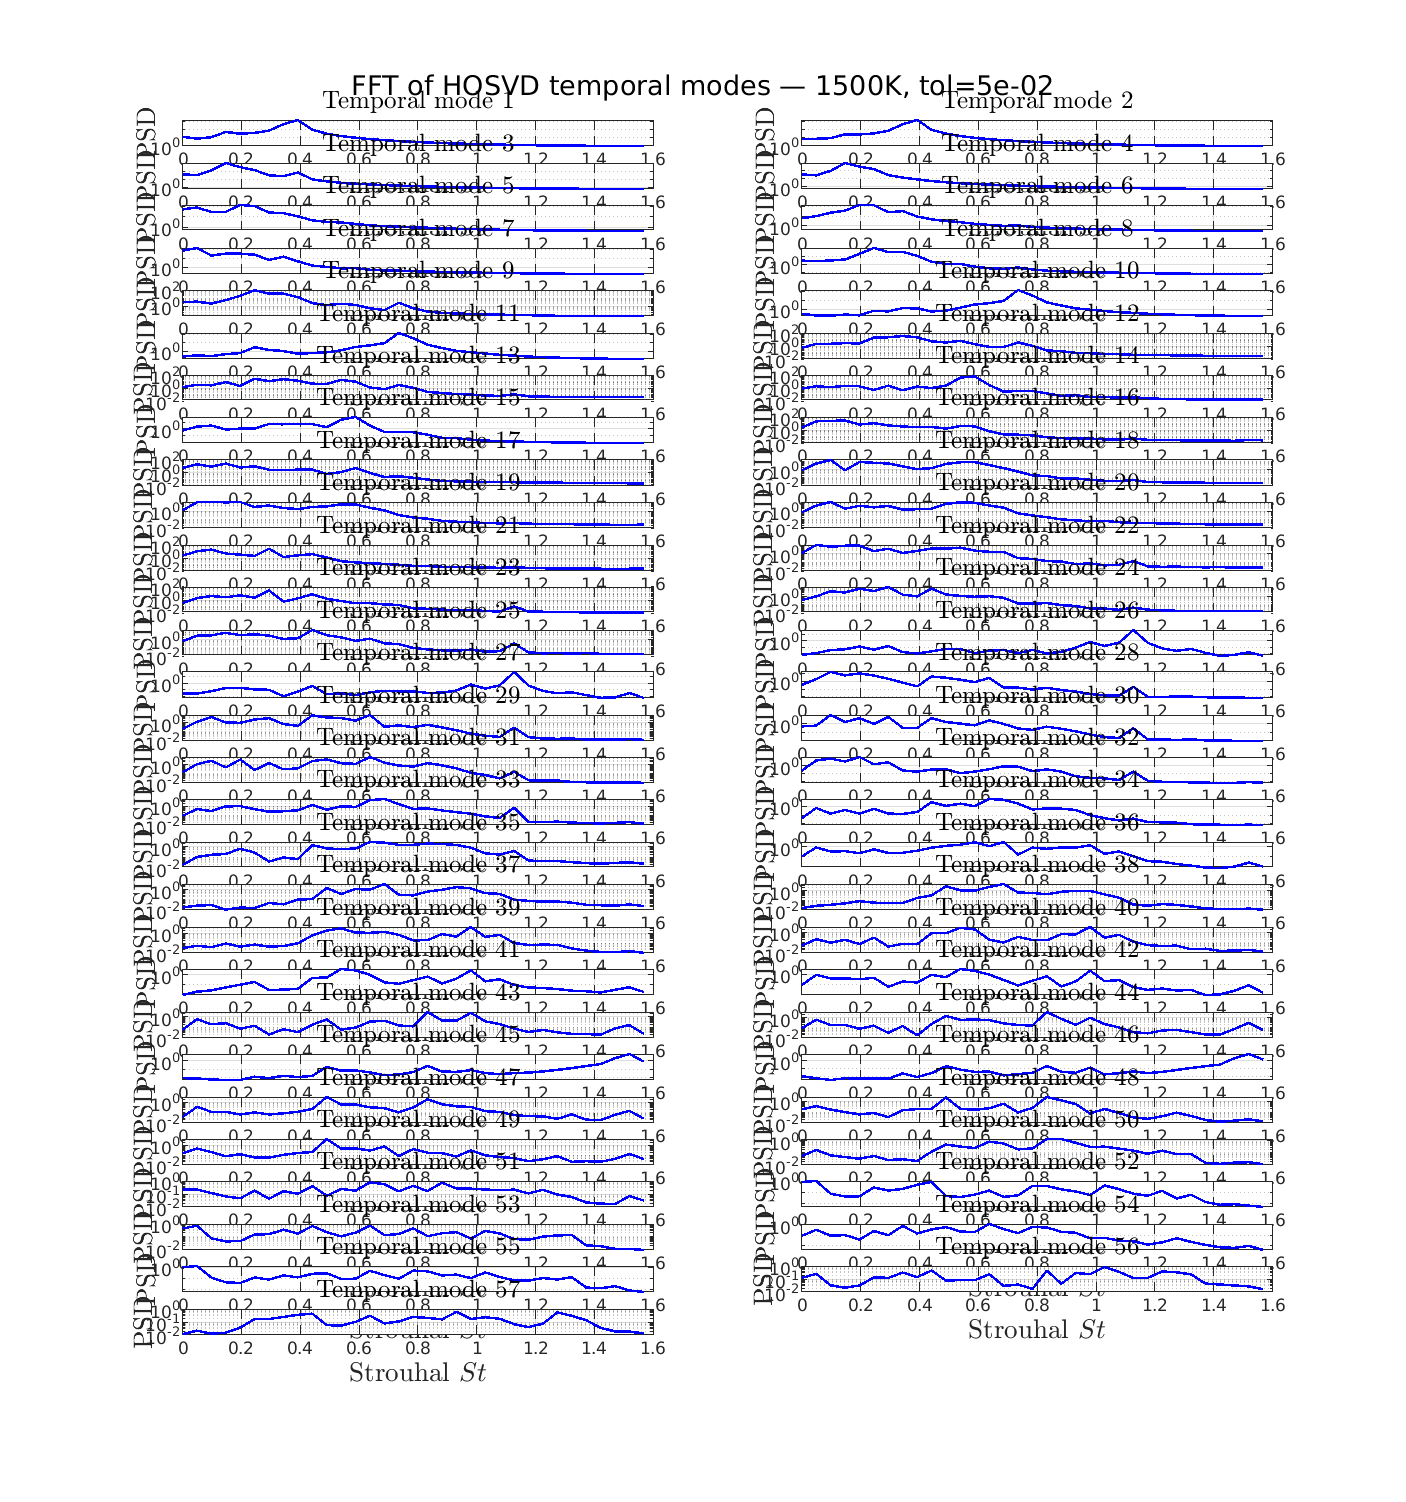
\includegraphics[width=0.85\textwidth]{FFT_temporalmodes_1500K_tol5e-02.png}
    \caption{FFT spectra of HOSVD temporal modes for the 1500~K dataset at $\varepsilon_\mathrm{tol} = 5\times10^{-2}$. Each panel shows the power spectral density of one retained temporal mode as a function of Strouhal number $St$.}
    \label{fig:fft_temporal}
\end{figure}
\FloatBarrier

\subsection{DMD Mode Amplitude Spectrum}

Figure~\ref{fig:amplitude_spectrum} shows the DMD mode amplitudes as a function of Strouhal number for a selection of parameter combinations ($d = 35, 40, 45$; $\varepsilon_\mathrm{tol} = 5\times10^{-2}$ and $7\times10^{-2}$). Several dominant peaks emerge consistently across parameter settings, notably near $St \approx 0.21$--$0.25$, $St \approx 0.37$--$0.42$, and a high-amplitude mode near $St \approx 0.42$. The robustness of these peaks across different $d$ and $\varepsilon_\mathrm{tol}$ values indicates that they represent genuine physical features of the flame dynamics rather than artefacts of the decomposition parameters.

\begin{figure}[htbp]
    \centering
    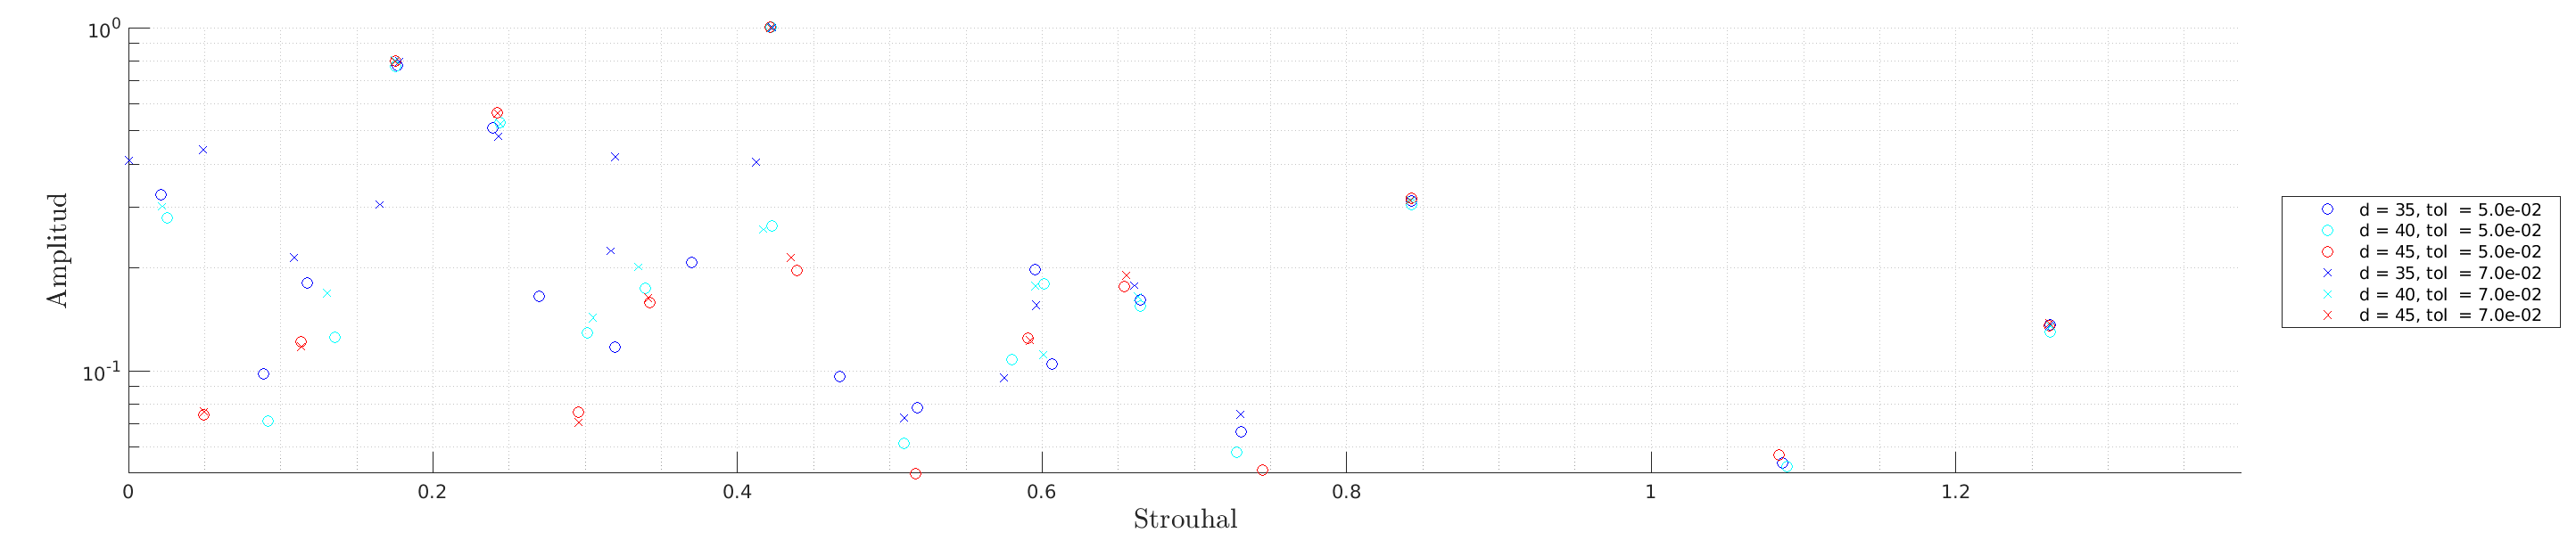
\includegraphics[width=\textwidth]{PLOT_CASE_1.png}
    \caption{DMD mode amplitudes as a function of Strouhal number for the 1500~K dataset across selected parameter combinations. Circles and crosses distinguish different tolerances; colours distinguish different delay values $d$.}
    \label{fig:amplitude_spectrum}
\end{figure}
\FloatBarrier

\subsection{Spatial DMD Modes}

The spatial structure of the dominant DMD modes is examined for the configuration $d = 40$, $\varepsilon_\mathrm{tol} = 7\times10^{-2}$. Each mode is represented as a two-dimensional field over the $(x/h,\, y/h)$ domain for each of the six retained reactive scalar variables.

\subsubsection{Mode at $St = 0.214$}

\begin{figure}[htbp]
    \centering
    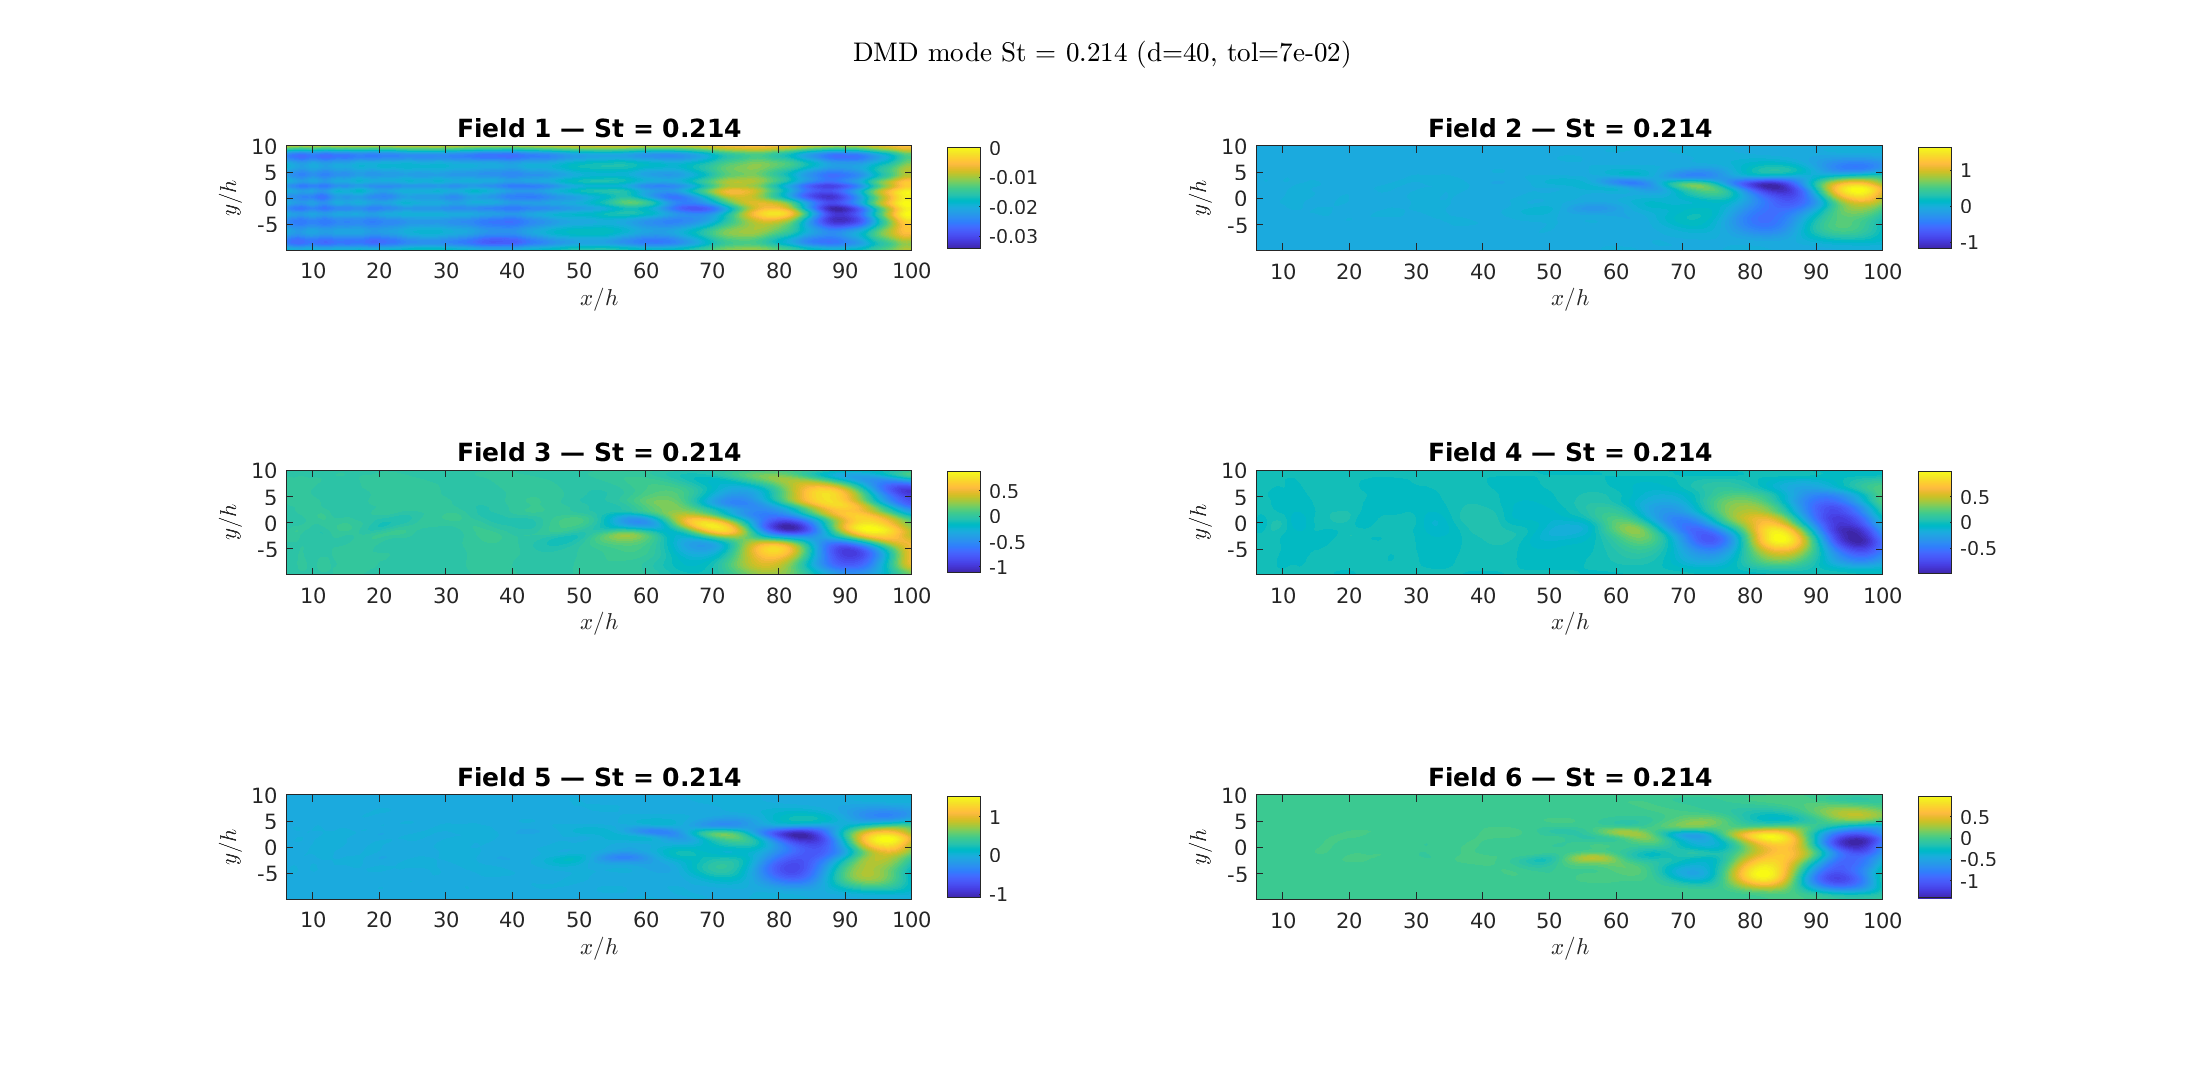
\includegraphics[width=\textwidth]{DMDmode_St0.21_d40_tol7e-02.png}
    \caption{Spatial DMD mode at $St = 0.214$ ($d=40$, $\varepsilon_\mathrm{tol}=7\times10^{-2}$). Each panel shows the real part of the mode for one reactive scalar field over the streamwise--cross-stream plane.}
    \label{fig:mode_021}
\end{figure}

The mode at $St = 0.214$ (Figure~\ref{fig:mode_021}) is the lowest-frequency dominant structure identified in the spectrum. It exhibits elongated streamwise coherence with moderate cross-stream extent, consistent with a large-scale shear-layer oscillation. The spatial structure is concentrated in the downstream half of the domain, suggesting that this mode is associated with the convective growth and saturation of the Kelvin--Helmholtz instability of the mixing layer.
\FloatBarrier

\subsubsection{Mode at $St = 0.244$}

\begin{figure}[htbp]
    \centering
    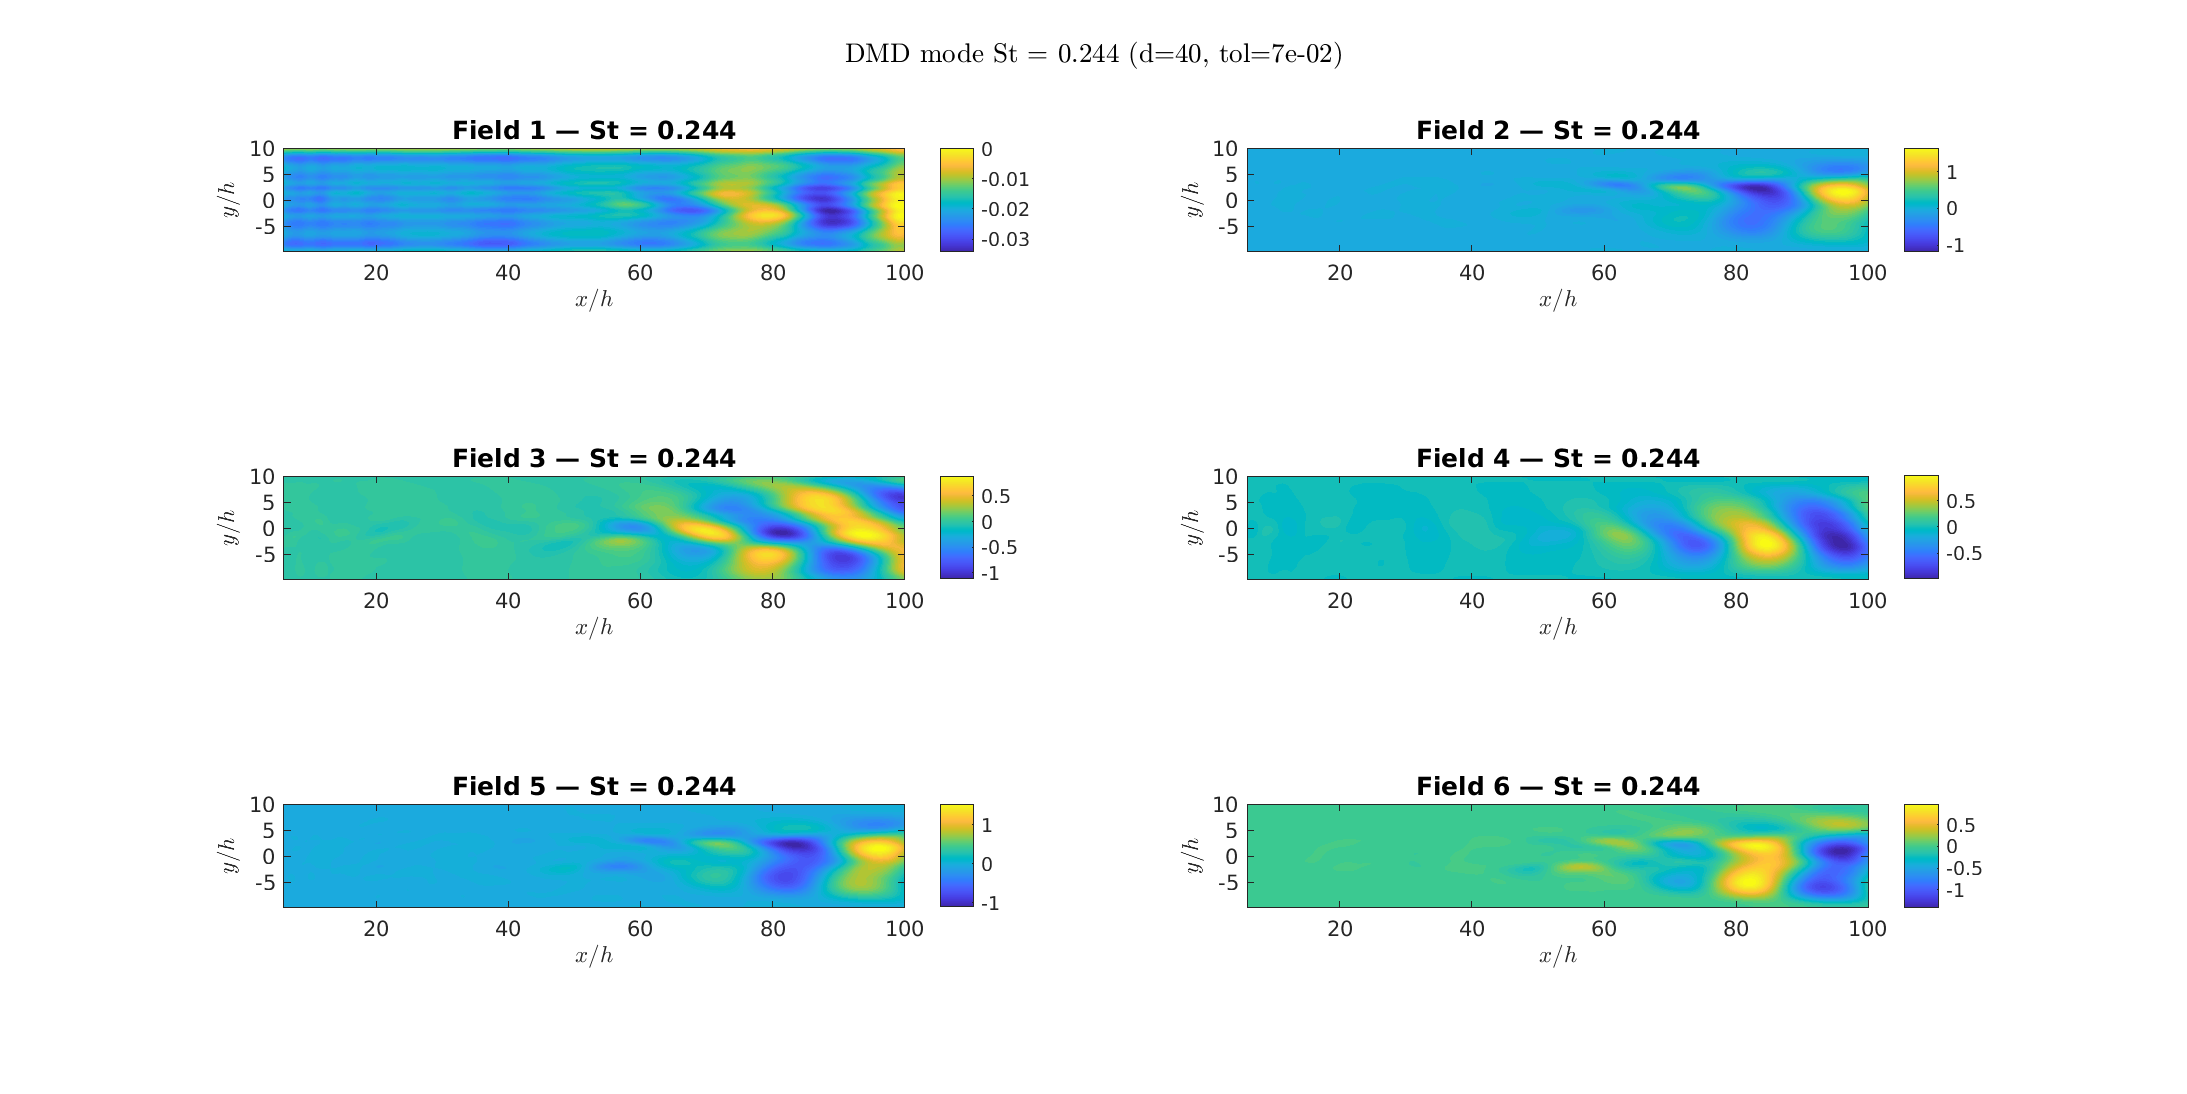
\includegraphics[width=\textwidth]{DMDmode_St0.24_d40_tol7e-02.png}
    \caption{Spatial DMD mode at $St = 0.244$ ($d=40$, $\varepsilon_\mathrm{tol}=7\times10^{-2}$).}
    \label{fig:mode_024}
\end{figure}

The mode at $St = 0.244$ (Figure~\ref{fig:mode_024}) presents a spatial organisation similar to the $St = 0.214$ mode but with a shorter streamwise wavelength. This suggests a harmonic or sub-harmonic relationship between the two structures, possibly linked to vortex pairing in the developing shear layer.
\FloatBarrier

\subsubsection{Mode at $St = 0.271$}

\begin{figure}[htbp]
    \centering
    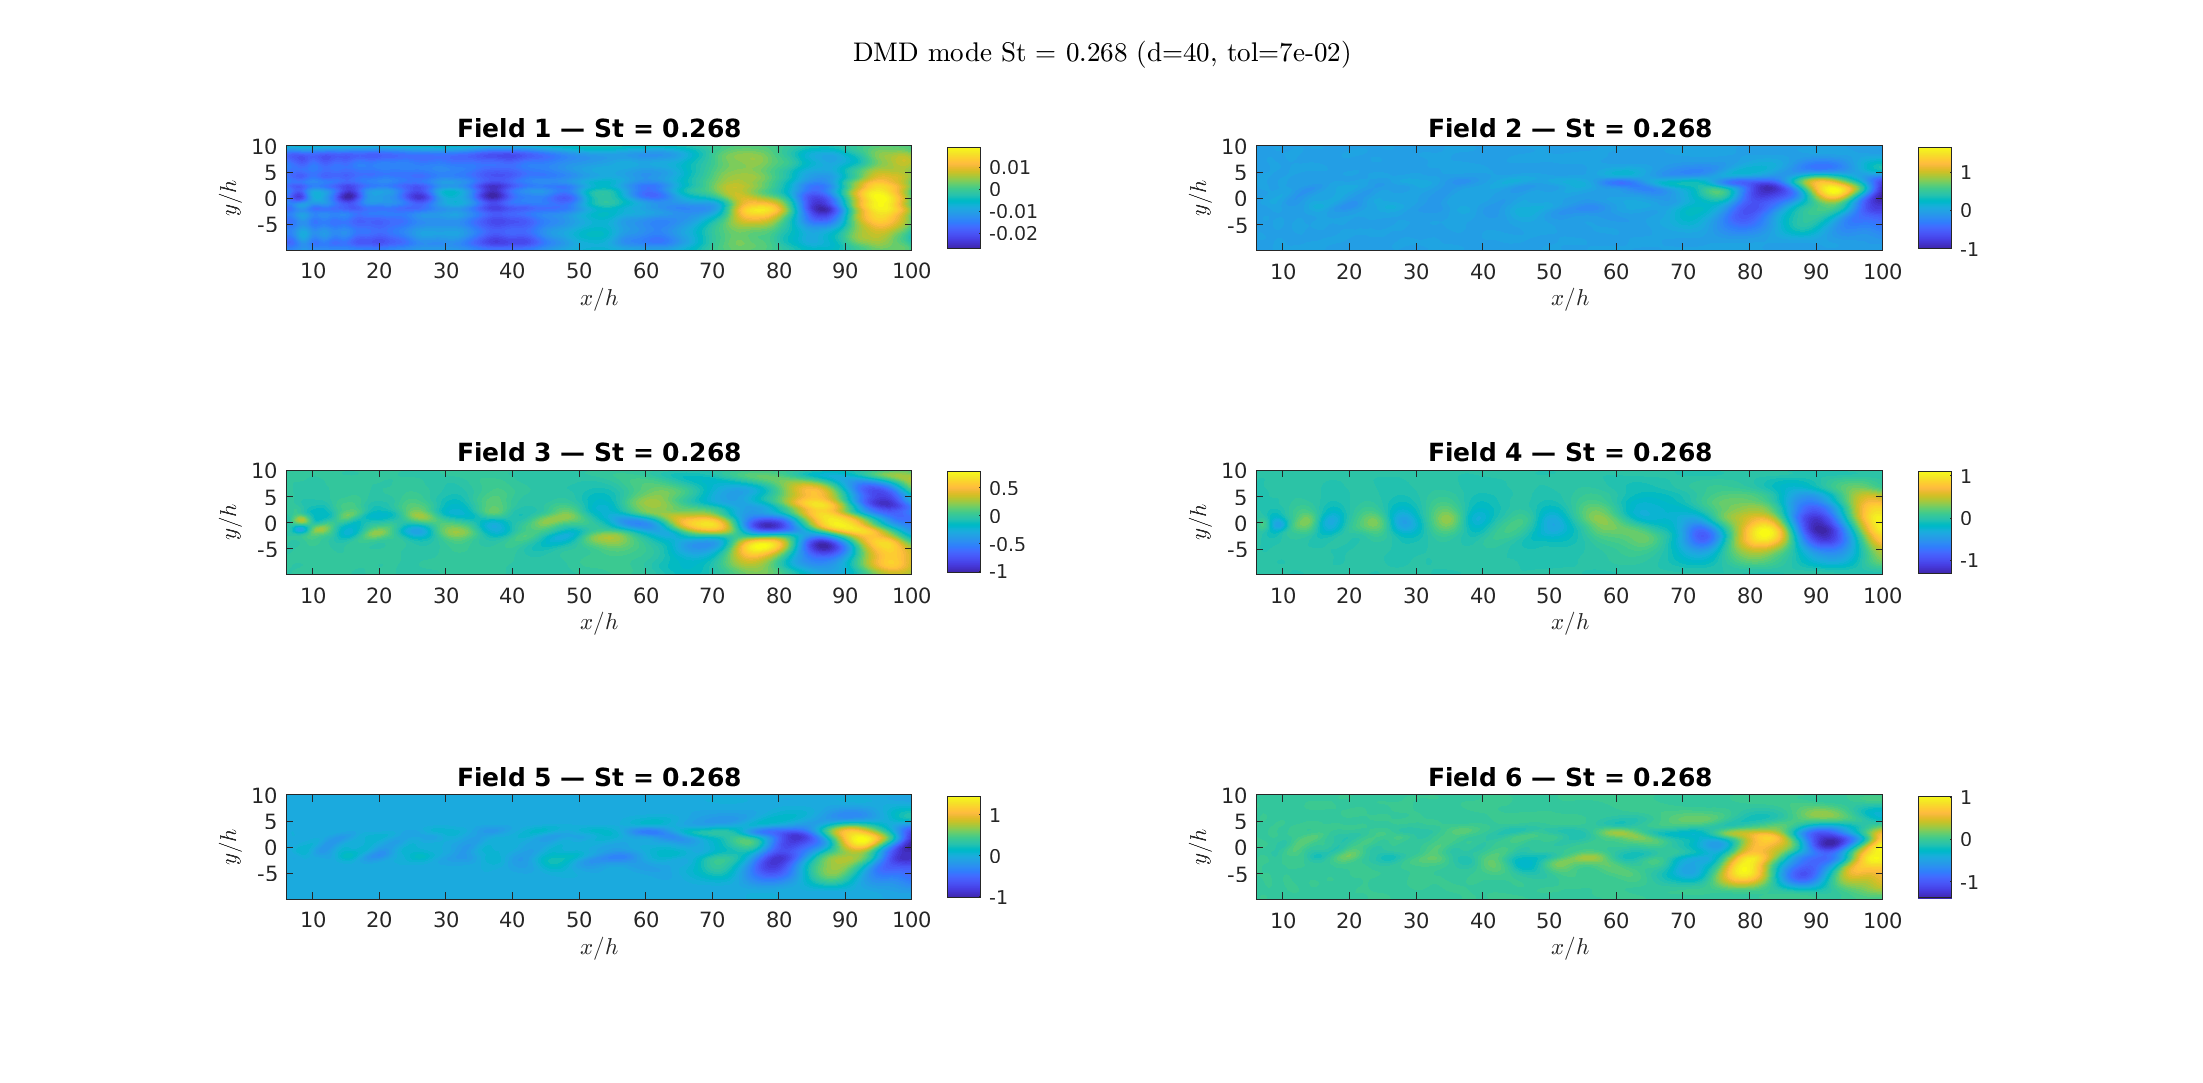
\includegraphics[width=\textwidth]{DMDmode_St0.27_d40_tol7e-02.png}
    \caption{Spatial DMD mode at $St = 0.271$ ($d=40$, $\varepsilon_\mathrm{tol}=7\times10^{-2}$).}
    \label{fig:mode_027}
\end{figure}

The mode at $St = 0.271$ (Figure~\ref{fig:mode_027}) shows a transition towards finer spatial scales, with increased cross-stream modulation compared to the lower-frequency modes. This structure may be associated with secondary instabilities developing on top of the primary shear-layer roll-up.
\FloatBarrier

\subsubsection{Mode at $St = 0.371$}

\begin{figure}[htbp]
    \centering
    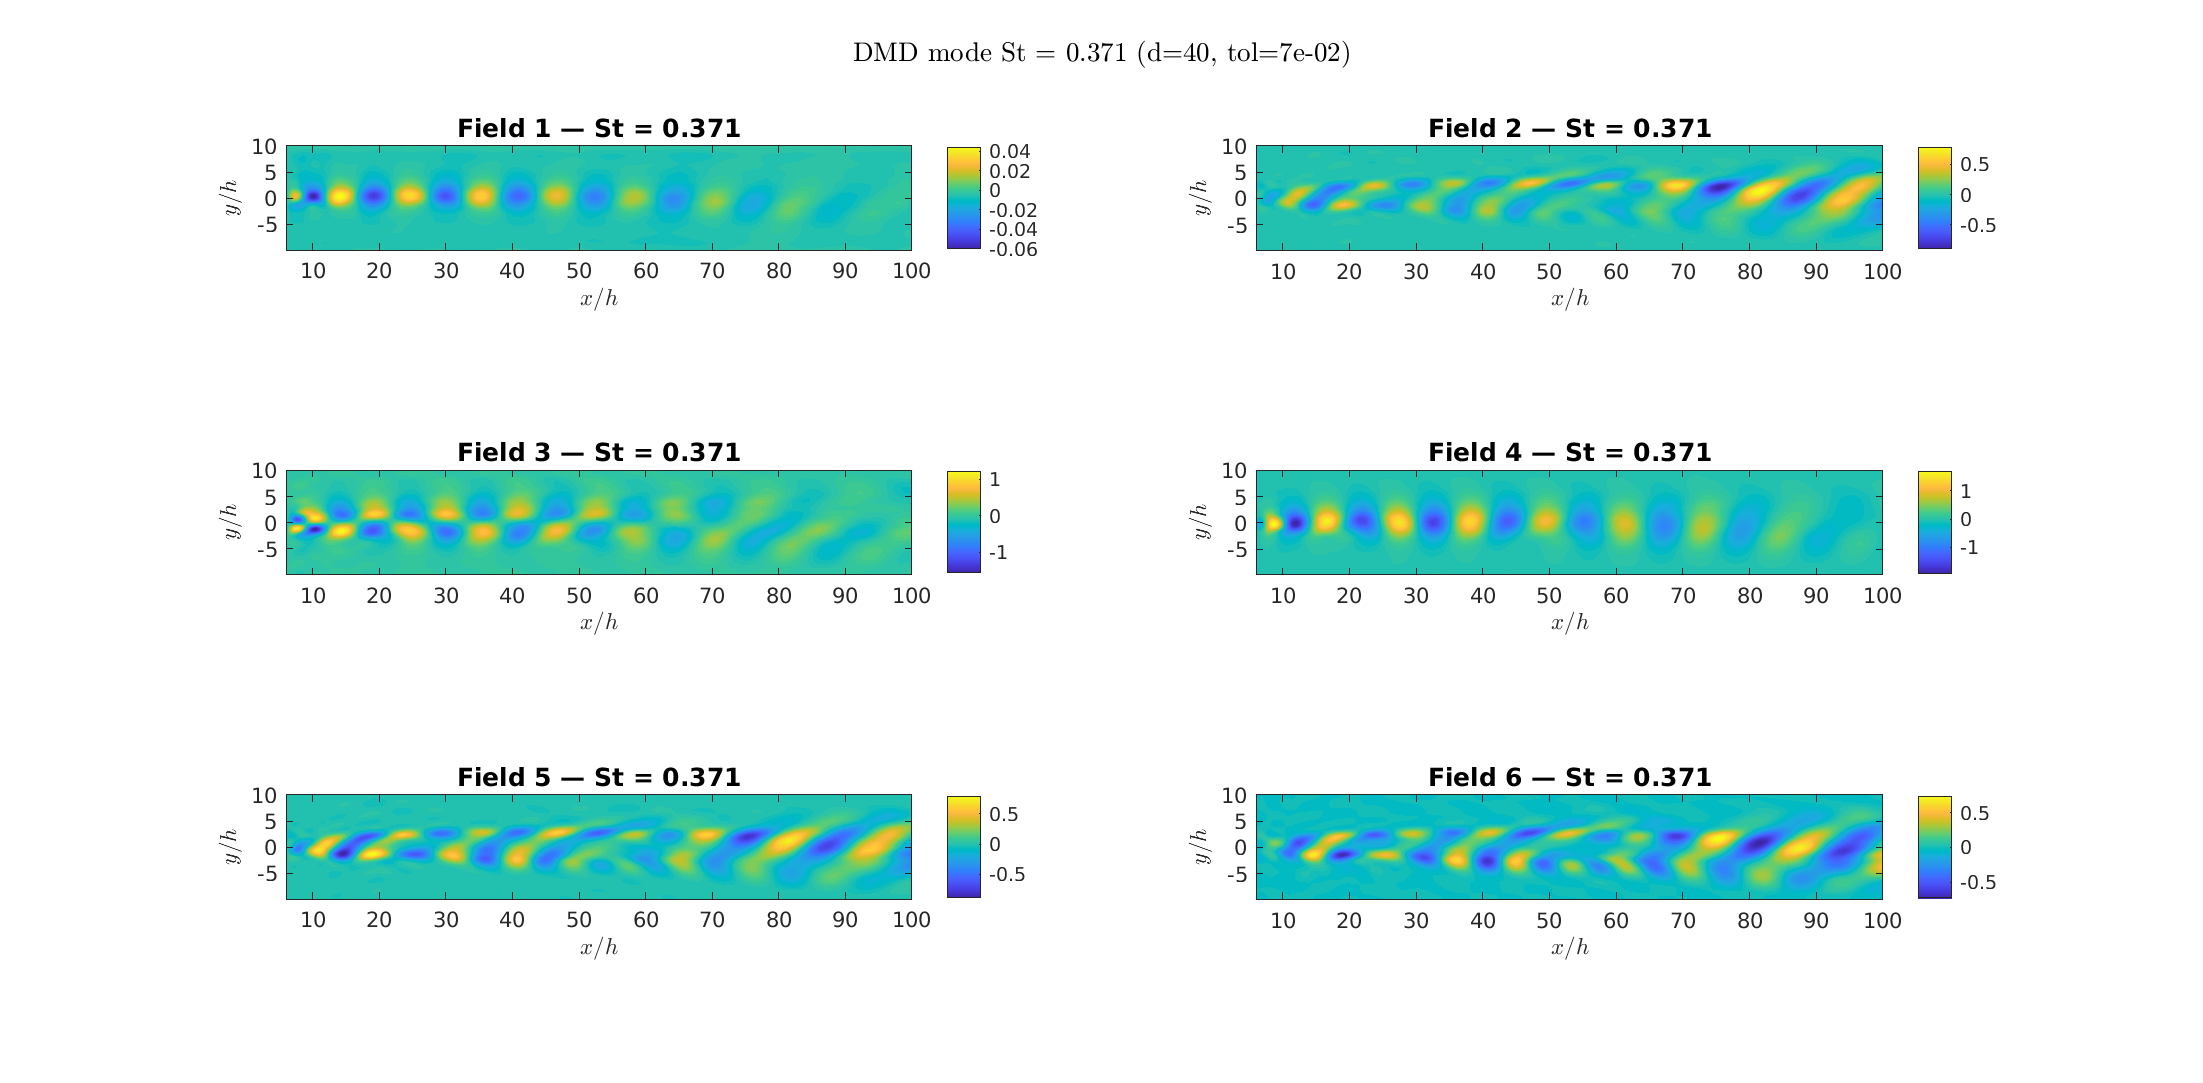
\includegraphics[width=\textwidth]{DMDmode_St0.37_d40_tol7e-02.png}
    \caption{Spatial DMD mode at $St = 0.371$ ($d=40$, $\varepsilon_\mathrm{tol}=7\times10^{-2}$).}
    \label{fig:mode_037}
\end{figure}

At $St = 0.371$ (Figure~\ref{fig:mode_037}), the mode displays a pronounced alternating pattern in both the streamwise and cross-stream directions. This spatial signature is characteristic of higher-frequency coherent structures embedded in the shear layer, and the increased spatial frequency relative to the lower-$St$ modes suggests a more rapid temporal evolution associated with smaller vortical structures.
\FloatBarrier

\subsubsection{Mode at $St = 0.422$}

\begin{figure}[htbp]
    \centering
    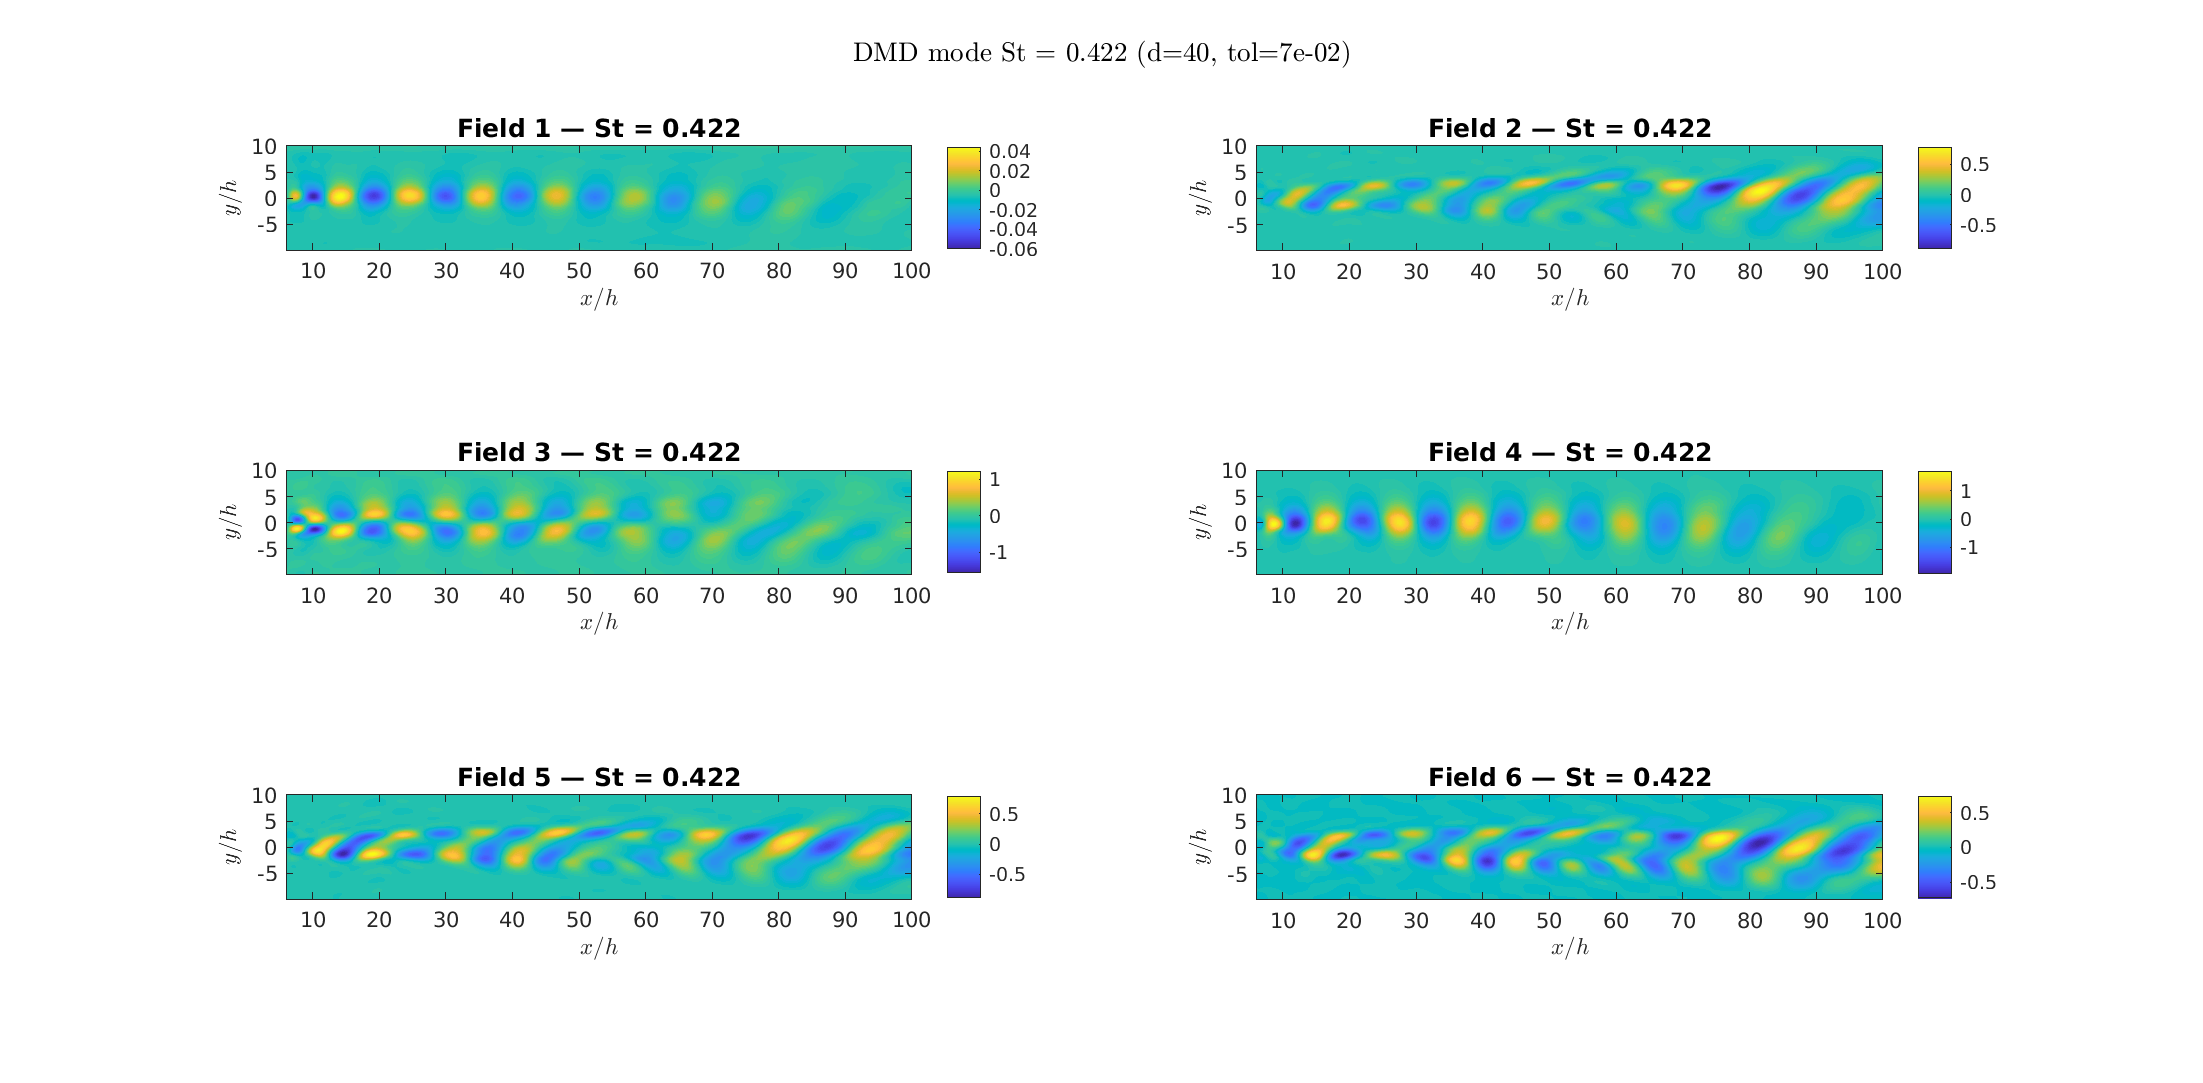
\includegraphics[width=\textwidth]{DMDmode_St0.42_d40_tol7e-02.png}
    \caption{Spatial DMD mode at $St = 0.422$ ($d=40$, $\varepsilon_\mathrm{tol}=7\times10^{-2}$). This is the highest-amplitude mode in the spectrum.}
    \label{fig:mode_042}
\end{figure}

The mode at $St = 0.422$ (Figure~\ref{fig:mode_042}) is the dominant mode in terms of amplitude (Figure~\ref{fig:amplitude_spectrum}). Its spatial structure closely resembles that of the $St = 0.371$ mode but with a slightly higher spatial frequency. The simultaneous presence of both modes with comparable amplitudes suggests a coupled dynamics between these two Strouhal numbers, possibly arising from nonlinear interactions within the reactive shear layer.
\FloatBarrier

\subsection{Discussion}

The mdHODMDit algorithm successfully extracts a set of physically coherent spatio-temporal modes from the high-dimensional DNS tensor without requiring any reshaping of the data into matrix form. The HOSVD stage effectively compresses the information while preserving the multi-variable structure of the dataset, enabling the subsequent HODMD to operate on a low-dimensional representation that retains the essential dynamics. The iterative loop further refines the decomposition by removing noise and non-coherent contributions, converging to a self-consistent set of modes.

The dominant frequencies identified in the Strouhal range $St \approx 0.2$--$0.5$ are consistent with convective instability mechanisms in non-premixed mixing layers. The spatial modes show a clear progression from large-scale shear-layer structures at low $St$ to finer-scale alternating patterns at higher $St$, reflecting the multi-scale nature of the reactive flow dynamics. The robustness of these features across the parameter sweep provides confidence in their physical significance.


% ---------------- Bibliography ----------------
\bibliographystyle{plain}
\bibliography{references}

\end{document}
